\apendice{Plan de Proyecto Software}
\section{Introducción}

En la fase de planificación se hace un análisis de las diferentes fases y tareas que
se abordan en el proyecto, estimando así el trabajo, el tiempo y los costes económicos
que supondrán el desarrollo de este.

Para llevar a cabo esta planificación, se analiza en proyecto en su totalidad y se 
divide en partes. Dependiendo de la metodología que hayamos escogido, se hará de una 
manera u otra, bien sea a través de sprints, fases en cascada, etc.

Como hay varias cosas que se deben estimar, podemos dividir esta etapa en:
\begin{itemize}
  \tightlist
  \item\textbf{Planificación temporal}: en esta parte se llevará a cabo el análisis de las distintas
  fases que formarán el desarrollo del proyecto y se hará una planificación de la 
  duración de las mismas, así como la diferencia entre el tiempo estimado y el real.
  \item\textbf{Estudio de viabilidad}: este a su vez lo dividiremos en viabilidad económica y viabilidad legal, ya que tendremos que tener en cuenta las herramientas código abierto y las librerías que sean de pago en caso de que las hubiera.
\end{itemize}

\newpage
\section{Planificación temporal}
Como se ha indicado previamente, la planificación temporal comprende todas las fases que
forman parte del desarrollo del proyecto. 

Debido a la metodología elegida (modelo en cascada con ruta crítica), se ha dividido 
el desarrollo en diferentes etapas, cada una de distinta duración en función del tamaño
o del número de tareas de cada una. 

Las diferentes etapas elegidas son:
\begin{itemize}
\item Fase 0: Organización previa y configuración principal de la aplicación.
\item Fase 1: Layout, inicio de sesión, registros y perfiles de los usuarios.
\item Fase 2: Directorio de usuario y gestión de currículum.
\item Fase 3: Edición, borrado, clonación y exportación de currículum.
\item Fase 4: Gestión de currículum para administradores.
\item Fase 5: Publicaciones en la página principal.
\item Fase 6: Administración y mantenimiento de usuarios.
\item Fase 7: Despliegue de la aplicación en servidor con una máquina virtual.
\item Fase 8: Mejoras y extras.
\item Fase 9: Documentación.
\end{itemize}

Cada fase se corresponde con una \emph{milestone} en el repositorio del proyecto, de manera
que se separan las tareas por cada tipo de etapa.
A continuación, se detallarán cada una de las fases mencionadas.

\subsection{Fase 0: Organización previa y configuración principal de la aplicación}
Esta fase, al ser la primera de todas, comprende toda la etapa de análisis y 
construcción previa de la aplicación. Esta etapa, a su vez, se divide en dos secciones,
que han sido separadas en análisis/primeros pasos.

Por lo tanto, las dos subsecciones de esta fase serían:
\begin{itemize}
\tightlist
\item Fase 0.1: Organización previa y análisis.
\item Fase 0.2: Configuración inicial de la aplicación.
\end{itemize}

La primera sección, la de análisis, busca, por un lado, las necesidades del proyecto en cuanto
a entorno, librerías, lenguajes y dependencias y, por otro lado, el diseño de la base de datos.

La lista de las principales tareas que se han llevado a cabo en esta sección son:
\begin{itemize}
\tightlist
\item Análisis y diseño de la base de datos (modelos, tablas, campos...).
\item Dependencias del proyecto.
\item Creación del proyecto y de los modelos.
\item Configuración de la aplicación con la cadena de conexión.
\item Primera migración a base de datos.
\item Manejo de excepciones y ``logs'' del proyecto con Serilog y ExceptionHandlerMiddleware.
\end{itemize}

Para esta primera parte, la duración estimada ha sido de 3 horas, y la duración real ha sido de 3.5 horas.

En la segunda sección se comienza a diseñar la aplicación en cuanto a vistas y estructura interna,
configurando el layout principal (del que dependen el resto de vistas), hojas de estilos,
importar el estilo base de la aplicación, etc.
\begin{figure}
    \centering
    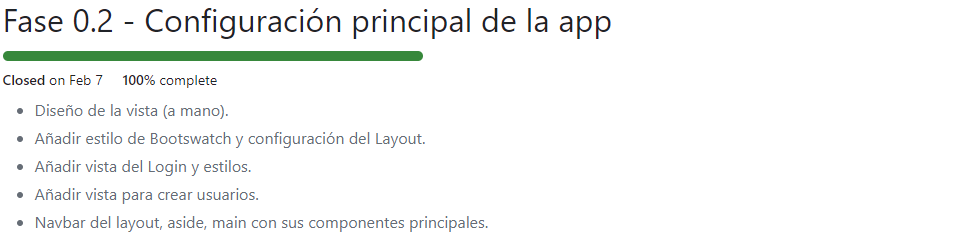
\includegraphics[width=\linewidth]{Fase0}
    \caption{Milestone de la fase 0}
\end{figure}
\newpage
La lista de las principales tareas que se han llevado a cabo en esta sección son:
\begin{itemize}
\tightlist
\item Diseño de las vistas principales.
\item Creación de las clases para los modelos de la base de datos.
\item Añadir el estilo principal de la aplicación.
\item Crear la vista del inicio de sesión (base).
\item Crear la vista para registrar usuarios (base).
\item Creación del layout principal con sus elementos.
\end{itemize}

El diseño inicial que se ha cogido como base para la aplicación se ha obtenido de 
\href{https://bootswatch.com/}{Bootswatch}\footnote{Bootswatch: https://bootswatch.com/}. Esta página tiene diseños gratuitos de
Bootstrap para su uso en cualquier aplicación web.

El diseño que se ha utilizado ha sido \href{https://bootswatch.com/flatly/}{\emph{Flatly}}\footnote{Diseño Flatly: https://bootswatch.com/flatly/}.

Para esta segunda parte, la duración estimada ha sido de 5 horas, y la duración real ha sido de 5 horas.

Al final, el total de tiempo estimado en esta fase cero ha sido de 8 horas, y el resultado
final ha sido de una duración de 8 horas y media, debido a diversos problemas con las versiones
de las dependencias, que ha alargado más la primera parte.

\subsection{Fase 1: \emph{Layout}, \emph{login}, registros y perfiles de los usuarios}
En esta fase, después de haber organizado la parte inicial de la aplicación, se comienza a llevar
a cabo el desarrollo principal del proyecto. 

Esta parte, en específico, comprende la gestión básica de los usuarios, creando la pantalla principal, el perfil, el registro de usuarios y el inicio de sesión correcto de los usuarios registrados.

Al igual que en el caso anterior, esta fase se divide en varias secciones:
\begin{itemize}
\tightlist
\item Fase 1.1: Configuración total del layout.
\item Fase 1.2: Inicio de sesión y registro de usuarios.
\item Fase 1.3: Configuración del perfil de los usuarios.
\end{itemize}

En la primera sección tenemos la configuración del layout. En esta parte se realizarán todas las
redirecciones a las diferentes vistas a las que se podrán acceder a través de este, el navbar
y la paginación de la pantalla principal.
\begin{figure}
    \centering
    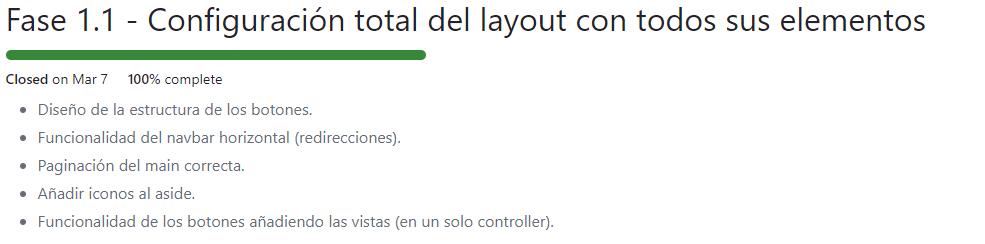
\includegraphics[width=\linewidth]{Fase1-1}
    \caption{Milestone de la fase 1.1}
\end{figure}

De esta forma, las tareas que se realizan son:
\begin{itemize}
\tightlist
\item Redirecciones al resto de vistas.
\item Añadir botones funcionales con el aside lateral.
\item Paginación de la pantalla principal.
\item Añadir iconos a las diferentes funciones.
\end{itemize}

Para esta primera parte, la duración prevista fue de una hora, y el tiempo real ha sido de una 
hora y media, debido a que la paginación del main se ha realizado a medida.

En la segunda sección se llevará a cabo el inicio de sesión y el registro de nuevos usuarios.
\begin{figure}
    \centering
    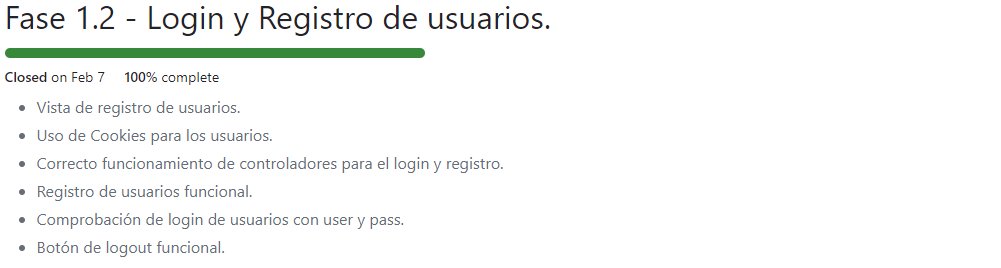
\includegraphics[width=\linewidth]{Fase1-2}
    \caption{Milestone de la fase 1.2}
\end{figure}
\newpage

La división de las tareas ha sido la siguiente:
\begin{itemize}
\tightlist
\item Vista del registro de usuarios completa y funcional.
\item Uso de ``cookies'' y variables de sesión para los usuarios.
\item Controladores para el inicio de sesión y registro.
\item Registro funcional de usuarios.
\item Comprobación de la funcionalidad del inicio de sesión.
\item Vista del inicio de sesión finalizada.
\item Logout de usuarios y limpieza de las \emph{cookies}.
\end{itemize}

Para las cookies he utilizado una dependencia que crea un objeto del modelo de base de datos.
En este objeto se puede añadir los atributos que se requieran, y se devuelve a la vista
para la permanencia de los datos. Gracias a este objeto, se pueden rellenar de datos las
variables de sesión para poder acceder a ellos en cualquier momento desde el controlador.

El tiempo estimado para estas tareas ha sido de 8 horas, y la duración final ha sido de 7 horas.

Por último, la tercera sección de esta fase comprende la configuración del perfil 
de los usuarios, y las tareas que se han llevado a cabo son:
\begin{itemize}
\tightlist
\item Vista para el perfil de los usuarios.
\item Creación de un modelo para guardar los datos principales.
\item Cambio de biografía y foto de perfil del usuario.
\item Cambio de la contraseña del usuario.
\end{itemize}

\begin{figure}
    \centering
    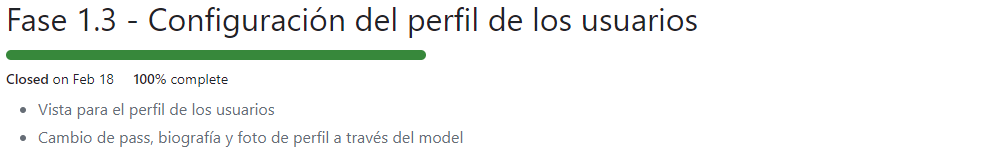
\includegraphics[width=\linewidth]{Fase1-3}
    \caption{Milestone de la fase 1.3}
\end{figure}
Para esta sección se había considerado una duración de 5 horas, pero debido a la dificultad del
guardado de la foto de perfil en el servidor, se ha realizado en 6 horas.

La duración real total de esta fase ha sido de 14 horas y media.

\subsection{Fase 2: Directorio de usuario y gestión de currículos}
Esta fase comienza con la gestión de currículos desde el punto de vista del usuario, y se divide
en dos vistas: la vista del directorio y la vista de los currículos.

Como es una aplicación orientada al usuario, el directorio ofrece una gestión de archivos para este,
aunque por ahora solo se implementa un gestor de notas cortas.

Esta fase también tiene dos divisiones:
\begin{itemize}
\tightlist
\item Fase 2.1: Directorio del usuario y notas.
\item Fase 2.2: Comienzo con la gestión del currículum.
\end{itemize}

La primera parte tiene como objetivo crear la vista del directorio y hacer la funcionalidad
de las notas de los usuarios, de forma que tenemos las siguientes tareas:
\begin{itemize}
\tightlist
\item Vista para el directorio de los usuarios.
\item Botón para añadir nuevas notas.
\item Visualización de todas las notas del usuario en sesión.
\item Editar, borrar y ver el contenido de las notas.
\end{itemize}

\begin{figure}
    \centering
    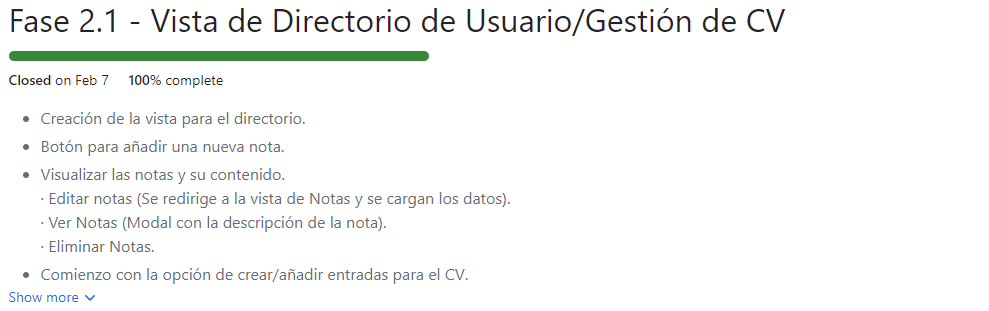
\includegraphics[width=\linewidth]{Fase2-1}
    \caption{Milestone de la fase 2.1}
\end{figure}

La duración de esta sección se ha estimado en 5 horas, que es lo que se ha invertido al final.

La segunda parte inicia la gestión de los currículos, y las tareas asignadas han sido:
\begin{itemize}
\tightlist
\item Creación de la vista para visualizar los currículos.
\item Botón para añadir un nuevo currículum.
\item Tabla con los iconos necesarios para los currículos.
\end{itemize}

\begin{figure}
    \centering
    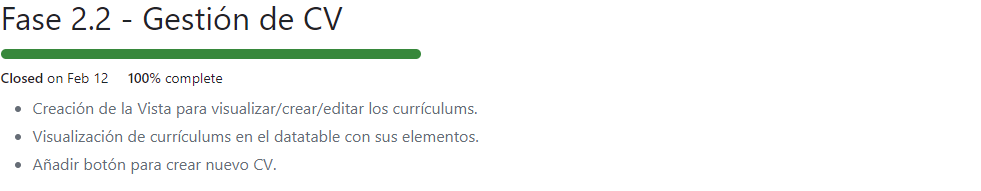
\includegraphics[width=\linewidth]{Fase2-2}
    \caption{Milestone de la fase 2.2}
\end{figure}

Para esta parte se han calculado 4 horas y se ha realizado en 3 horas. En total, el tiempo
estimado en esta fase ha sido de 9 horas y el tiempo invertido total ha sido de 8 horas, reduciendo
así el tiempo estimado en una hora.

\subsection{Fase 3: Edición, borrado, clonación y exportación de currículos}
Esta es la etapa más larga y en la que más tiempo se ha invertido en total, ya que es el 
núcleo o funcionalidad principal de la aplicación, que es la gestión de currículos.

Esta etapa se divide en varias secciones, igual que las anteriores:
\begin{itemize}
\tightlist
\item Fase 3.1: Edición de currículos.
\item Fase 3.2: Borrado de currículos.
\item Fase 3.3: Clonación de currículos.
\item Fase 3.4: Exportación a PDF.
\end{itemize}

La primera sección es el desarrollo principal de la gestión. Una vez se crea un currículum
y a parece en la tabla de la vista de los currículos, al dar al icono de editar se nos
abrirá una vista con las diferentes partes que comprenden un currículum para llenarlo de 
información. 

Toda la información del currículum se divide en un acordeón de html que tiene varios desplegables:
\begin{itemize}
\tightlist
\item 1: Información principal del usuario (nombre y apellidos, email, número, profesión...).
\item 2: Información académica.
\item 3: Idiomas.
\item 4: Experiencia laboral.
\item 5: Aptitudes y logros.
\end{itemize}

\begin{figure}
    \centering
    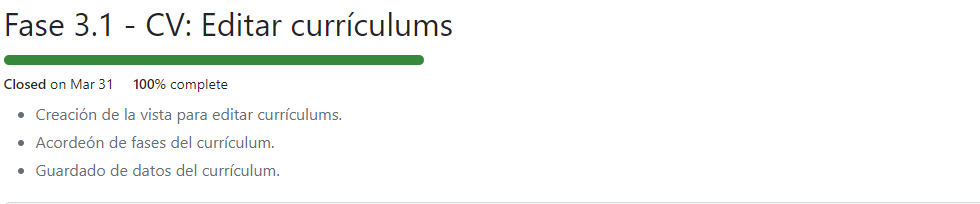
\includegraphics[width=\linewidth]{Fase3-1}
    \caption{Milestone de la fase 3.1}
\end{figure}

Todas estas partes se pueden rellenar y guardar por igual, no son pasos sucesivos sino que están 
en la misma vista, para facilitar el guardado de los datos. Cada cambio en esta pantalla modifica
los datos del currículum.

Las tareas asignadas han sido:
\begin{itemize}
\tightlist
\item Creación de la vista con el acordeón.
\item Acordeón con las diferentes pasos de información al completo.
\item Guardado de todos los datos.
\end{itemize}

Todo lo que comprende esta vista, al ser demasiado grande, se ha valorado en unas 30 horas 
de trabajo, ya que en muchos casos la información es dinámica (pueden haber varias entradas
para idiomas, experiencia laboral y formación académica), de modo que se ha tenido que 
controlar el poder añadir varias entradas con JavaScript.

El tiempo total invertido ha sido de 33 horas finalmente.

La segunda parte se centra en el borrado de currículos existentes. A través de la tabla de
los currículos, hay un icono de una papelera con el que podremos borrar en su totalidad un
currículum.

Al hacer click sobre este botón, se nos mostrará un modal para confirmar la operación, y, al aceptar, el currículum se elimina de la base de datos y desaparece.

\begin{figure}
    \centering
    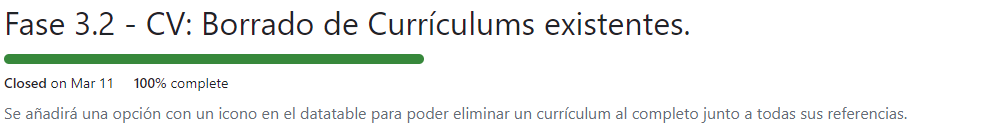
\includegraphics[width=\linewidth]{Fase3-2}
    \caption{Milestone de la fase 3.2}
\end{figure}

Como ha sido una sección corta, las tareas han sido la creación del modal para aceptar y la
funcionalidad del botón, por lo que se ha calculado una duración de 2 horas, y el tiempo real
invertido ha sido de finalmente 3 horas.

En tercer lugar, tenemos la clonación de currículos. Esta utilidad permite, desde la tabla
de los currículos, la posibilidad de copiar un currículum y crear uno idéntico, con los mismos 
datos. 

Esta funcionalidad se propuso para agilizar la creación de currículos similares y que contengan
al final los mismos datos.

\begin{figure}
    \centering
    
\includegraphics[width=\linewidth]{Fase3-3}
    \caption{Milestone de la fase 3.3}
\end{figure}

El tiempo estimado para la clonación fue de 4 horas y se realizó en 6 horas, debido a 
que había cierta dificultad para clonar las fotos del usuario.


Para finalizar con esta fase tenemos la exportación a PDF de los currículos. Se ha utilizado la
librería de Rotativa PDF, que permite exportar un objeto PDF desde el controlador, creando
a través de los datos del modelo y con una vista como plantilla, un documento en formato
PDF de los datos que se deseen.

Las tareas necesarias en esta fase han sido:
\begin{itemize}
\tightlist
\item Creación de la vista de la plantilla del pdf.
\item Llenar de datos el modelo que se va a utilizar.
\item Configuración de la librería y añadir los archivos principales.
\item Creación del objeto de Rotativa y hacer la exportación.
\end{itemize}

\begin{figure}
    \centering
    
\includegraphics[width=\linewidth]{Fase3-4}
    \caption{Milestone de la fase 3.4}
\end{figure}

Además, para hacer la exportación se ha tenido en cuenta un formato específico, que es el
formato europeo de currículos. Este formato es el genérico utilizado en toda Europa en 
cuanto a empresas y administraciones públicas se refiere.

Para la realización de esta fase se han estimado 12 horas, y la duración final ha sido de 13 horas.

En el total de toda esta gestión de currículos, la duración prevista ha sido de 50 horas y el
tiempo total invertido ha sido de 55 horas.

\subsection{Fase 4: Gestión de currículos para administradores}
Esta fase no ha sido dividida en varias secciones debido a que se hace todo a través de la
misma pantalla.



Las diferencias entre las pantallas de los usuarios administradores y los normales son:
\begin{itemize}
\tightlist
\item El usuario no administrador solo puede ver sus currículos (y realizar el resto
de operaciones sobre su propio currículum).
\item El usuario administrador tiene un listado de todos los currículos que existen
en la base de datos y puede exportarlos a PDF o ver sus datos principales desde la
propia vista.
\item El usuario administrador, además, tiene varios campos por los que puede filtrar
los currículos para hacer una búsqueda más específica, si se requieren documentos
que cumplan ciertos requisitos (de idioma, rango de edad, etc.).
\end{itemize}

En esta fase, las tareas realizadas han sido las siguientes:
\begin{itemize}
\tightlist
\item Creación de la vista para la gestión de los currículos.
\item Listado de todos los documentos en una tabla con sus funcionalidades de ver y exportar.
\item Filtros para las búsquedas a través de varios de los campos.
\item Redirecciones y restricciones entre usuarios normales y administradores.
\item Funcionalidad de los filtros y los botones de ver y exportar.
\end{itemize}

\begin{figure}
    \centering
    
\includegraphics[width=\linewidth]{Fase4}
    \caption{Milestone de la fase 4}
\end{figure}

Para esta fase, se ha hecho una previsión de 18 horas, y la duración final de esta etapa ha sido
de 20 horas.

\subsection{Fase 5: Publicaciones en la página principal}
La página principal es la primera vista que vemos nada más iniciamos sesión en la aplicación.
En esta página se encuentras las publicaciones, que tienen un formato de red social y que 
funcionan como anuncios que pueden aportar información al usuario.

Junto a las publicaciones se implementan unos filtros de búsqueda, de forma similar a los
que hay en la gestión de currículos de los administradores.

Las tareas realizadas en esta fase han sido:
\begin{itemize}
\tightlist
\item Creación de la vista para las publicaciones.
\item Estructura de las publicaciones.
\item Filtros para la búsqueda de publicaciones.
\item Opción para añadir una publicación.
\end{itemize}

\begin{figure}
    \centering
    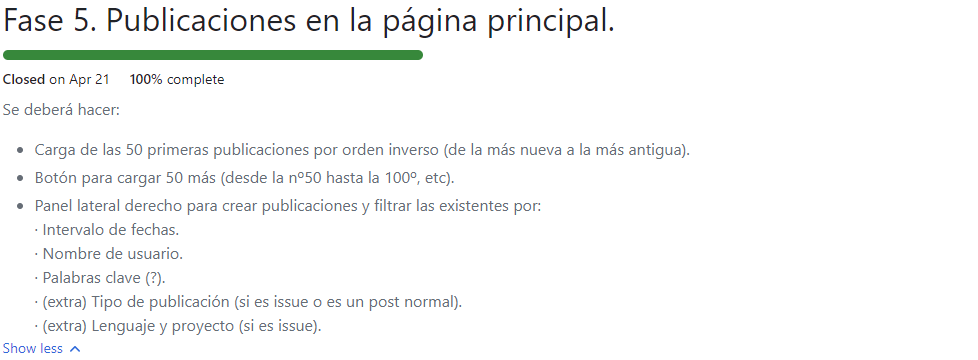
\includegraphics[width=\linewidth]{Fase5}
    \caption{Milestone de la fase 5}
\end{figure}

El tiempo estimado para la realización de estas tareas ha sido de 6 horas, completándolo todo
en un tiempo final de 6 horas.

\subsection{Fase 6: Administración y mantenimiento de usuarios}
El mantenimiento de usuarios es muy similar a la vista de gestión de currículos de los
administradores. 

Por un lado tenemos una lista de todos los usuarios en una tabla y por
otro podemos cargar y visualizar los datos de los usuarios para cambiarlos.

Las tareas realizadas en esta fase han sido:
\begin{itemize}
\tightlist
\item Creación de la vista para el mantenimiento de usuarios.
\item Tabla con los usuarios.
\item Visualización de los datos de los usuarios a través de un botón.
\item Edición de los datos de los usuarios.
\end{itemize}

\begin{figure}
    \centering
    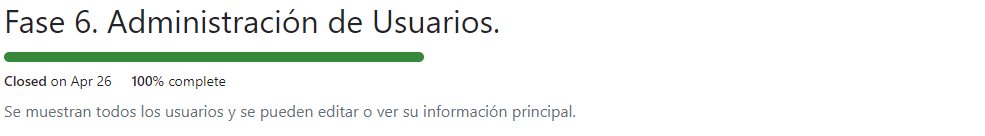
\includegraphics[width=\linewidth]{Fase6}
    \caption{Milestone de la fase 6}
\end{figure}

La duración prevista para el desarollo de esta fase ha sido de 7 horas y se ha completado en 8
horas, aumentando así el tiempo estimado en una hora.

\subsection{Fase 7: Despliegue de la aplicación en servidor con una máquina virtual}
El despliegue de la aplicación es la más importante para las pruebas y la solución
final. Como se ha explicado previamente, el servidor web se creará a través de una
máquina virtual de Windows 10, que genera un servidor local a través del IIS Express.

El proceso de construcción del servidor tiene los siguientes pasos o tareas:
\begin{itemize}
\tightlist
\item 1. Se crea la máquina virtual de Windows 10.
\item 2. Se instancian el SQL Server y el SQL Management Studio y se añade la base de datos.
\item 3. Se configura el IIS que genera la instancia del servidor de la web.
\item 4. Se publica la aplicación en un directorio y se apunta a este desde el IIS.
\item 5. Se genera una dirección local para acceder a ella desde un navegador.
\end{itemize}
La máquina virtual se exportará como un archivo en formato ``.ova'' que se importará
directamente a VirtualBox o VMWare (en función de la aplicación que se use para 
gestionar las máquinas virtuales).

\begin{figure}
    \centering
    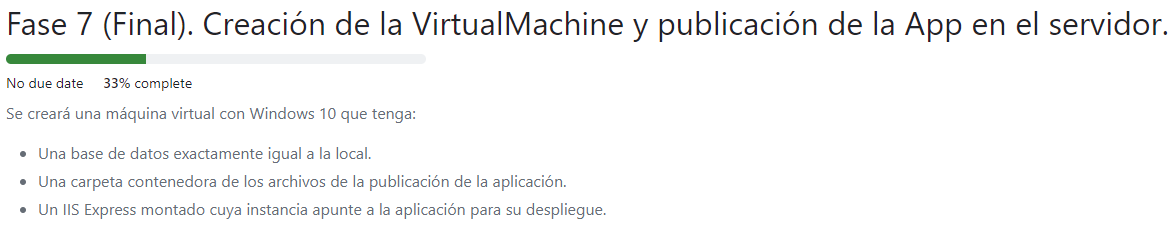
\includegraphics[width=\linewidth]{Fase7}
    \caption{Milestone de la fase 7}
\end{figure}

La máquina virtual tiene ciertas necesidades a la hora de instalarla, por lo tanto dependerá 
del equipo en el que lo instalemos. Debido a esto, hay que comprobar que el sistema anfitrión cumpla unos requerimientos de memoria, procesadores, etc.

Para ello, se aportan los datos de la máquina virtual, que son los siguientes:
\begin{table}[h]
	\centering
	\begin{tabular}{lc }
		\toprule
		\textbf{Característica}    & \textbf{Valor}\\
		\toprule
  	\text{Sistema Operativo}                & Windows 10 Home    \\
		\text{Memoria Virtual}                  & 50 GB   \\
		\text{Memoria RAM}                      & 4 GB \\
		\text{Procesadores}                     & 3-4 procesadores\\
		\bottomrule
	\end{tabular}
	\caption{Datos Máquina Virtual}
\end{table}

Para crear la máquina virtual y configurar todo lo necesario ha sido necesario invertir 20 horas de trabajo.


\subsection{Fase 8: Mejoras y extras}
La fase de mejoras es un añadido que está fuera del alcance del proyecto (esto se explicará
más adelante). En esta etapa se han añadido las tareas que, o bien eran las menos prioritarias,
o bien estaban estimadas como mejoras a la aplicación una vez estuviera terminada.

En esta fase podemos ver tareas como las siguientes:
\begin{itemize}
\tightlist
\item Mejoras y cambios en el diseño general de la aplicación.
\item Añadir el registro de usuarios en el inicio de sesión.
\item Añadir campo booleano activo a varias tablas para su mantenimiento.
\item Añadir contactos dentro de la aplicación.
\item Respuestas a publicaciones y notificaciones.
\item Añadir campos y atributos nuevos a los currículos.
\item Filtros nuevos en la gestión de usuarios y currículos para los administradores.
\end{itemize}

\begin{figure}
    \centering
    
\includegraphics[width=\linewidth]{Fase8}
    \caption{Milestone de la fase 8}
\end{figure}

Como las mejoras están fuera del alcance del proyecto, no se estima una duración exacta,
ya que son tareas que se proponen a futuro y debido a que forman una lista que puede
alargarse con más procesos. La duración total ha sido de 35 horas, contando la revisión y corrección de errores.

\subsection{Fase 9: Documentación}
La documentación es la última parte del desarrollo de este proyecto, pero es algo que se ha ido haciendo de manera progresiva a lo largo de este. En esta fase se incluye la documentación de los siguientes apartados:
\begin{itemize}
\tightlist
\item Anexos (este documento).
\item Memoria.
\item Manuales de instalación, del programador y de usuario.
\item Casos de uso.
\item Diagramas E/R de los modelos.
\end{itemize}

Todos los materiales que se han querido documentar están tanto en la memoria como en 
los anexos. Al principio se quería incluir los casos de uso y los manuales en archivos
por separado, pero al final se han acabado incluyendo en los anexos.

En la documentación tenemos las siguientes tareas:
\begin{itemize}
\tightlist
\item Búsqueda de información bibliográfica y preparación de los documentos.
\item Obtención de imágenes, tablas y figuras que aportan información.
\item Formato y estructura de la memoria y anexos correctos.
\item Documentar todos los puntos de la estructura de la memoria y de los anexos.
\item Tablas para los casos de uso.
\item Compilación de imágenes de ejemplo para los manuales de instalación y usuario.
\item Revisión de errores y avisos con el editor de Overleaf antes de la entrega.
\end{itemize}

La duración valorada para la memoria ha sido la más larga de todas las fases, siendo esta de
45-48 horas. 

En la tabla \ref{duracionDoc} se muestra la duración total de cada una de las partes de la documentación.
\begin{table}
	\centering
	\begin{tabular}{ lr }
		\toprule
		\textbf{Documentación}    & \textbf{Horas invertidas}\\
		\toprule
		\text{Memoria}                          & 25 h  \\
		\text{Anexos (A-D)}                     & 40 h \\
		\text{Manuales}                         & 20 h \\
		\text{Casos de uso}                     & 20 h \\
        \text{Imágenes y figuras}               & 5 h \\
		\text{Investigación}                    & 15 h \\
		\text{Revisión y corrección}            & 5 h \\
		\bottomrule
		\textbf{Total horas invertidas}    & 130 h\\
	\end{tabular}
	\caption{Duración total de la documentación}
    \label{duracionDoc}
\end{table}


\begin{table}
	\centering
	\begin{tabular}{lr}
		\toprule
		\textbf{Fase}    & \textbf{Horas invertidas}\\
		\toprule
		\text{Fase 1: Análisis y configuraciones}         & 30 h  \\
		\text{Fase 2: Directorio de usuarios}             & 8 h \\
		\text{Fase 3: Edición de currículos}                    & 55 h \\
		\text{Fase 4: Administración de currículos}             & 20 h \\
        \text{Fase 5: Publicaciones en index}             & 6 h \\
        \text{Fase 6: Administración de usuarios}         & 8 h \\
        \text{Fase 7: Despliegue servidor}                & 20 h \\
        \text{Fase 8: Mejoras, extras y revisión}         & 35 h \\
        \text{Fase 9: Documentación}                      & 130 h \\
		\bottomrule
		\textbf{Total horas invertidas}    & 312 h\\
	\end{tabular}
	\caption{Horas invertidas totales de las fases}
    \label{duracionTot}
\end{table}
Finalmente, la duración total de todas las fases se muestra en la tabla \ref{duracionTot}.

\newpage
\section{Estudio de viabilidad}
\subsection{Viabilidad económica}
La aplicación se desarrolla en un entorno y marco de trabajo de código abierto, ya que se utilizan herramientas software como SQL Management Studio y Visual Studio Community 2022 para su desarrollo, herramientas que ofrece Microsoft de forma gratuita.

Además para el despliegue de la web se utilizará una máquina virtual con Windows 10 de forma local, por lo que no hará falta alojarla en un servidor de pago, solo en el contexto de la empresa se deberá contemplar este último punto, para añadir el proyecto como una nueva instancia al servidor de esta junto al resto de aplicaciones internas.

Debido a este último punto, se hará un análisis realista de los gastos económicos que supondrían
para una empresa, divididos en varios tipos de costes:
\begin{itemize}
\tightlist
\item Costes de personal.
\item Costes de material y derivados de la empresa.
\end{itemize}

Se va a suponer que la duración del proyecto han sido las 300 horas que se recogen en la 
guía docente del TFG a la que incluimos 60 horas de planificación en la empresa, instalación
y pruebas, de manera que distribuido equitativamente en jornadas laborales de 8 horas al día durante 5 días a la semana, tenemos:

360 horas / (8 horas * jornada) = 40 jornadas

Tenemos 40 jornadas, que con 5 a la semana son aproximadamente dos meses de trabajo.

\subsubsection{Coste de personal}
El coste del personal equivaldrá al salario de la persona que realice el proyecto. En 
este caso vamos a considerar que solo tenemos un trabajador y que se considera la nómina de la tabla \ref{tablaNomina}.

\begin{table}
	\centering
	\begin{tabular}{lr }
		\toprule
		\textbf{Conceptos}    & \textbf{Costes}\\
		\toprule
		\text{Salario Base}                     & 950€   \\
		\text{Convenios}                        & 250€ \\
		\text{Complementos}                     & 250€ \\
		\text{Total devengo (bruto)}            & 1450€ \\
		\text{Retenciones (IRPF 15\% y otros)}  & 250€ \\
		\text{Seguridad Social (28,3\%)}        & 406€ \\
		\bottomrule
		\textbf{Total en dos meses}    & 3712€\\
	\end{tabular}
	\caption{Coste de personal}
    \label{tablaNomina}
\end{table}

\subsubsection{Coste de material y general de la empresa}
En cuanto al material necesario para la realización del proyecto, tenemos, por un lado, el 
equipo o el dispositivo en el que se realizará (hardware) y, por otro lado, el software
necesario que tendrá este equipo. 

Por otro lado debemos analizar los gastos internos de la empresa, tales como alquiler de oficinas
y su mantenimiento (luz, agua, Internet, etc.), servidores y otras licencias.

De esta forma, podemos observar el costo total en la tabla \ref{tablaCostosEmpresa}.

\begin{table}
	\centering
	\begin{tabular}{lr }
		\toprule
		\textbf{Conceptos}    & \textbf{Costes}\\
		\toprule
		\text{Portátil}                         & 900€   \\
		\text{Windows 10 Home}                  & 145€ \\
        \text{Servidor (mes)}                   & 125€ \\
        \text{Oficina + mantenimientos (mes)}   & 1000€ \\
        \text{Internet}                         & 180-200€ \\
        \text{Dominio de GitLab Ultimate (mes)} & 100€ \\
		\bottomrule
		\textbf{Total}    & 2450-2470€\\
	\end{tabular}
	\caption{Coste material y general de la empresa}
    \label{tablaCostosEmpresa}
\end{table}

\subsection{Viabilidad legal}
En esta segunda parte de la viabilidad, se describirán las licencias de las herramientas 
software utilizadas y de la documentación del proyecto.

Las herramientas, librerías y dependencias que se utilizan están sujetas a licencias. Una 
licencia es la forma en la que se distribuye el uso de un proyecto, una copia de este o su
documentación.

Incluso aunque una herramienta sea de código abierto, este está sujeto a una licencia que permite
que, de forma legal, el producto pueda ser utilizado de forma libre.

De esta forma se profundizará en las herramientas utilizadas y qué tipo de viabilidad 
legal tienen. Podemos dividirlo en dos secciones: por un lado tenemos las herramientas
con las que viene Visual Studio, o también llamadas herramientas internas. Por otro lado, las
herramientas externas, pueden ser, por ejemplo, \emph{Bootstrap}, \emph{Rotativa}, \emph{Datatables}, etc.

\subsubsection{Licencias Internas}
Como se ha mencionado previamente, las licencias internas serán:
\begin{itemize}
\tightlist
\item Dependencias del proyecto.
\item Librerías y paquetes NuGet.
\item Visual Studio.
\item Windows 10 Home.
\item SQL Management Studio.
\end{itemize}

Todas las licencias de las herramientas mencionadas forman parte de ``Microsoft Corporation'', ya
que son herramientas proporcionadas por Microsoft. Todas las anteriores, menos Windows 10, son
de uso libre.

Para crear la máquina virtual, el Windows 10 que se utiliza se crea a mano gracias a un 
archivo ``.iso'' que se genera gracias a una herramienta gratuita de Microsoft. Como no tiene
licencia, está sujeta a las mismas condiciones que Windows 10.

\subsubsection{Licencias Externas}
En cuanto a las licencias externas, tenemos:
\begin{itemize}
\tightlist
\item \emph{Bootstrap} y \emph{Bootswatch}.
\item \emph{Fontawesome}.
\item \emph{RotativaPDF}.
\item \emph{Datatables}.
\item \emph{JQuery}.
\end{itemize}

Las licencias de las librerías anteriores se muestran en la tabla \ref{tablaLicencias}.
\begin{table}
	\centering
	\begin{tabular}{lc}
		\toprule
		\textbf{Librería}    & \textbf{Licencia}\\
		\toprule
		\text{Bootstrap y Bootswatch}           & MIT license   \\
		\text{Fontawesome Fonts}                & SIL OFL 1.1 \\
  	\text{Fontawesome Code}                 & MIT license \\
    	\text{Fontawesome Documentation}        & CC BY 3.0 \\
        \text{JQuery}                           & MIT license \\
        \text{RotativaPDF}                      & MIT license \\
        \text{Datatables}                       & MIT license \\
		\bottomrule
	\end{tabular}
	\caption{Licencias de las librerías externas}
    \label{tablaLicencias}
\end{table}

\section{Licencias propias}
Hemos hablado de los diferentes tipos de licencias que se encuentran en las librerías y dependencias que se utilizan en el proyecto. En este apartado, veremos las licencias que tiene el proyecto en sí.

En el contexto de este proyecto, se van a dividir las licencias en función de cada una de las partes que componen este. Principalmente se usará la licencia de atribución, aunque se diferenciará su alcance entre código y documentación, teniendo como resultado el resumen de la tabla \ref{licenciasProyecto}.

Como el código que se desarrolla forma parte del desarrollo de un proyecto real de una empresa, se añade la particularidad de que sea no comercial, no siendo este el caso para el resto de los adjuntos de este proyecto.
\begin{table}
	\centering
	\begin{tabular}{lc }
		\toprule
		\textbf{Librería}    & \textbf{Licencia}\\
		\toprule
		\text{Código Interno}                   & CC BY-NC 4.0   \\
		\text{Máquina Virtual}                  & CC BY 4.0 \\
  	\text{Imágenes}                         & CC BY 4.0 \\
    	\text{Repositorio}                      & CC BY 4.0 \\
        \text{Documentación}                    & CC BY 4.0 \\
		\bottomrule
	\end{tabular}
	\caption{Licencias del proyecto}
    \label{licenciasProyecto}
\end{table}